\documentclass[a4,10pt]{aleph-notas}

%% --> Comandos adicionales
\usepackage{textcomp}
\usepackage{multirow}
\usepackage{booktabs}
\usepackage{longtable}
\usepackage{tikz}
\usepackage{colortbl}
\usepackage{csquotes}
\usepackage[sorting=none]{biblatex}
\usepackage{float}
\usepackage{multicol}
%% --> Paquetes comunes
\usepackage{listings}
\usepackage{enumitem}
\usepackage{lipsum}

%% --> Definición de colores
\definecolor{codegreen}{HTML}{A5BE00}
\definecolor{codegray}{rgb}{0.5,0.5,0.5}
\definecolor{codepurple}{rgb}{0.58,0,0.82}
\definecolor{backcolour}{rgb}{0.95,0.95,0.92}

%% --> Estilo para código
\lstdefinestyle{mystyle}{
    language={[LaTeX]TeX}, % lenguaje
    basicstyle=\bfseries\ttfamily,
    keywordstyle=\color{colordef},
    commentstyle=\color{codegreen},
    backgroundcolor=\color{gray!15},
    showstringspaces=false,
    flexiblecolumns=true,
    stringstyle=\ttfamily\color{blue},
    extendedchars=true,
    emph={rm,bf,it,sf}, %...
    literate=%
    *{$}{{{\color{red}\$}}}1 % produce $ en rojo
    {$$}{{{\color{red}\$\$}}}1
    {ó}{{\'o}}1%
    {í}{{\'i}}1%
    {á}{{\'a}}1%
    {ú}{{\'u}}1%
}

%% --> Selección de estilo para el código
\lstset{
    style=mystyle,escapeinside={(*@}{@*)}
}

% Blancos tipográficos
\newcommand{\mq}{\hspace{0.5em}}  %medio cuadratín
\newcommand{\tq}{\hspace{0.33em}} % un terio de cuadratín
\newcommand{\qq}{\hspace{0.25em}} % un cuarto de cuadratín
\newcommand{\fs}{\hspace{0.125em}} % un octavo de cuadratín
\newcommand{\ep}{\hspace{0.05em}} % espacio de pelo

%% --> Nota para el material
\newcommand{\informacion}{\noindent\footnotesize{\color{colordef}
El presente material fue desarrollado por:

\noindent
\textbf{Daniel Lara}

\emph{Facultad de Ciencias, Escuela Politécnica Nacional}

\noindent
\textbf{Andrés Merino}

\emph{Facultad de Ciencias Exactas y Naturales, Pontificia Universidad Católica del Ecuador}


\medskip\noindent
La versión actual del material es 1.2-(Mayo 2021). En caso de encontrar inconsistencias o errores en el presente material se pueden comunicar a \href{mailto:daniel.lara@alephsub0.org}{daniel.lara@alephsub0.org}. Para más información puedes visitar nuestro sitio web: \href{https://alephsub0.org}{alephsub0.org}

\medskip\noindent

\includegraphics[height=12pt]{Imagenes/cc.xlarge.png} 
\includegraphics[height=12pt]{Imagenes/by.xlarge.png} 
\includegraphics[height=12pt]{Imagenes/nc.xlarge.png} \begin{minipage}[c]{0.85\textwidth}Esta obra se encuentra bajo licencia Atribución-NoComercial-CompartirIgual 4.0 Internacional (CC BY-NC-SA 4.0) Para más información puede visitar: \url{https://creativecommons.org/licenses/by-nc-sa/4.0/}\end{minipage}

\medskip\noindent
Si deseas colaborar con el desarrollo de este material, el código fuente está disponible en:   
\url{https://github.com/alephsub0/LaTeX_Guias.git}. Cualquier aporte (\emph{Pull request}) será de gran ayuda para mejorar este material. 

%% -- > Aquí se incluyen los nombres de los colaborades de estas guias:
\medskip\noindent
Agradecimientos: Katheryn Yánes
}}

%%--> Formato para títulos
\titleformat{name=\section,numberless}[display]
  {\vspace*{-2mm}\bfseries\scshape\centering}
    {}{1ex}
    {\color{colortext}\large\titlerule\vspace{.05ex}
     }
    [\color{colortext}\vspace{.2ex}\titlerule]

\titleformat{\subsubsection}
    {\color{colortext}\normalsize\bfseries}
    {\thesubsubsection}{1em}{}
    
%% --> Datos de las guias
\universidad{Curso de \LaTeX}
\autor{Proyecto Alephsub0}
\materia{Introducción a \LaTeX}

%% --> Logos de las guias
\logouno[4.5cm]{Imagenes/Logos/LogoAlephsub0-02.png}
\longtitulo{0.6\linewidth}
\fecha{Abril de 2021}

%% --> Definición de la bibliografía
\addbibresource{Bibliografia.bib}

% -- Datos del libro
\nota{Guía 4}
\tema{Tablas, gráficos y bibliografía}

%% ---> Opciones adicionales
\newcommand{\Z}{\mathbb{Z}}
\newcommand{\N}{\mathbb{N}}

%% ---> Nuevos tipos de columnas
\newcolumntype{G}{>{\color{red}$\pm$}c}
\newcolumntype{C}[1]{>{\hspace{0pt}\centering\arraybackslash}m{#1}}
\newcolumntype{L}[1]{>{\raggedright\arraybackslash}m{#1}}

\titleformat{name=\section,numberless}[display]
  {\vspace*{-2mm}\bfseries\scshape\centering}
    {}{1ex}
    {\color{colortext}\large\titlerule\vspace{.05ex}
     }
    [\color{colortext}\vspace{.2ex}\titlerule]

\definecolor{micolor}{rgb}{.6,.5,.4}

%% --> comandos extra
\newcommand{\colorbar}[1]{\begin{tikzpicture} \draw [#1, line width=6](0,0) -- (.5,0); \end{tikzpicture}}

\newenvironment{caja}
    {
        \color{orange}
        \begin{tabular}{|p{0.9\textwidth}|}
        \hline \color{lapislazuli} 
    }
    { 
        \\ \hline
        \end{tabular} 
        \color{black}
    }

%%%%%%%%%%%%%%%%%%%%%%%%%%%%%%%%%%%%%%%%
%%%%%%%%%% Comienzo del documento
%%%%%%%%%%%%%%%%%%%%%%%%%%%%%%%%%%%%%%%%

\begin{document}

\encabezado

\informacion

\tableofcontents

\section{Tablas}

Para la creación de tablas usamos el ambiente \verb@tabular@, este tiene la siguiente estructura:

\begin{lstlisting}[frame=single]
\begin{tabular}{(*@\emph{formato}@*)}
(*@\emph{contenido de la tabla}@*)
\end{tabular}
\end{lstlisting}

El parámetro \emph{formato} especifica la alineación de la columna y los separadores que existen en ella; a continuación se encuentra una lista de los formatos de columna disponibles. Para la creación de una tabla es necesario especificar el número de columnas, mientras que no se requiere indicar el número de filas.

\begin{itemize}
    \item \verb@l@ alinea la columna a la izquierda;
    \item \verb@r@ alinea la columna a la derecha;
    \item \verb@c@ alinea la columna al centro;
    \item \verb@p{@\emph{longitud}\verb@}@ indica una columna con la longitud especificada, las unidades de medida disponibles son las especificadas en la guía 1.
    \item \verb@|@ indica una linea vertical de separación entre columnas.
\end{itemize}

Por otra parte, dentro del ambiente se usan los siguientes delimitadores:

\begin{itemize}
    \item \verb@&@ indica un cambio de columna;
    \item \verb@\\@ indica un salto de fila;
    \item \verb@\hline@ inserta una linea horizontal en la tabla;
    \item \verb@\cline{a-b}@ inserta una linea horizontal desde la columna $a$ a la columna $b$.
\end{itemize}

Un ejemplo para la generación de una tabla se encuentra a continuación:

\begin{lstlisting}[frame=single]
\begin{tabular}{|c|c|c|}
    \hline
    \textbf{Ciclo N$^{\circ}$} &	\textbf{Temperatura} & \textbf{Tiempo} \\ \hline
    1   & $245 \pm 5,5$ &	3 \\ \hline
    2	& $260 \pm 5,5$ &	8 \\ \hline
    3	& $275 \pm 5,5$ &	8 \\ \hline
    4	& $287 \pm 5,5$ &	8 \\ \hline
\end{tabular}
\end{lstlisting}

\begin{center}
  \begin{tabular}{|c|c|c|}
   \hline
    \textbf{Ciclo N$^{\circ}$} &	\textbf{Temperatura} & \textbf{Tiempo} \\ \hline
    1   & $245 \pm 5,5$ &	3 \\ \hline
    2	& $260 \pm 5,5$ &	8 \\ \hline
    3	& $275 \pm 5,5$ &	8 \\ \hline
    4	& $287 \pm 5,5$ &	8 \\ \hline
  \end{tabular}
\end{center}

Notemos que no es necesario incluir lineas verticales que separan a las columnas:

\begin{lstlisting}[frame=single]
\begin{tabular}{ccc}
    \toprule
    \textbf{Ciclo N$^\circ$} &	\textbf{Temperatura} & \textbf{Tiempo} \\ \midrule
    1   & $245 \pm 5,5$ &	3 \\[1mm]
    2	& $260 \pm 5,5$ &	8 \\[1mm]
    3	& $275 \pm 5,5$ &	8 \\[1mm]
    4	& $287 \pm 5,5$ &	8 \\
    \bottomrule
\end{tabular}
\end{lstlisting}


\begin{center}
  \begin{tabular}{|cc|c|}
   \hline
    \textbf{Ciclo N$^\circ$} &	\textbf{Temperatura} & \textbf{Tiempo} \\ \hline
    1   & $245 \pm 5,5$ &	3 \\
    2	& $260 \pm 5,5$ &	8 \\
    % 3	& $275 \pm 5,5$ &	8 \\[1mm]
    % 4	& $287 \pm 5,5$ &	8 \\
    \hline
  \end{tabular}
\end{center}

\subsection{Unir celdas}

Una de las primeras operaciones con las que nos podemos topar en la generación de una tabla es la necesidad de unir ciertas celdas. Para ello vamos a recurir al comando \verb@\multicolumn@, con la siguiente sintaxis

\begin{lstlisting}[frame=single]
\multicolumn{numero de columnas}{alineacion}{texto a colocar}
\end{lstlisting}

\subsection{Paquete \emph{booktabs}}

Este paquete se utiliza para tener algunas opciones adicionales para tablas como lineas con un grosor distinto para una mejor presentación.


\begin{lstlisting}[frame=single]
\begin{tabular}{cccccccc}
    \toprule
    \multirow{2}{*}{\textbf{COMPOSICION}} & \multicolumn{7}{c}{\textbf{FORMULACION}}\\ 
    \cmidrule{2-8}
    & \textbf{43} & \textbf{44} & \textbf{45} & \textbf{46} & \textbf{47} & 
    \textbf{48} & \textbf{49}\\ \midrule
    Poliamida-colageno    & 34,8  & 34,4 &	35  & 25  &	40  & 34,9  & 34,95\\[1mm] 
    Acrilamida            & 45	   & 45	  & 45	& 45  & 45	& 45	& 45   \\[1mm]
    Etilenglicol          & 10    & 10	  & 10	& 10  & 10	& 10	& 10   \\[1mm]
    Reticulante (DMEGL)   & 0,2   & 0,6  &--- & --- &	--- & 0,10	& 0,05 \\[1mm]
    Colageno hidrolizado  & 10	   & 10	  & 10	& 20  &5	& 10	& 10   \\[1mm]
    \bottomrule
\end{tabular}
\end{lstlisting}

\begin{center}
 \begin{tabular}{cccccccc}
  \toprule
  \multirow{2}{*}{\textbf{COMPOSICIÓN}} & \multicolumn{7}{c}{\textbf{FORMULACIÓN}}\\ 
  \cmidrule{2-8}
    & \textbf{43} & \textbf{44} & \textbf{45} & \textbf{46} & \textbf{47} & \textbf{48} & \textbf{49}\\ \midrule
  Poliamida-colágeno    & 34,8  & 34,4 &	35  & 25  &	40  & 34,9  & 34,95\\[1mm] 
  Acrilamida           & 45	   & 45	  & 45	& 45  & 45	& 45	& 45   \\[1mm] \bottomrule
%   Etilenglicol          & 10    & 10	  & 10	& 10  & 10	& 10	& 10   \\[1mm]
%   Reticulante (DMEGL)   & 0,2   & 0,6  &	--- & --- &	--- & 0,10	& 0,05 \\[1mm]
%   Colágeno hidrolizado  & 10	   & 10	  & 10	& 20  &5	& 10	& 10   \\[1mm]
 \end{tabular}
\end{center}

\subsection{Paquete \emph{tabularx}}

Muchos de los ambientes y herramientas de \LaTeX{} se ven limitados por sus caracteristicas. En el caso de las tablas, para agregar más funciones vamos a incluir el paquete \verb@tabularx@

\subsubsection{Nuevos tipos de columnas}

Una de las principales ventajas del paquete \verb@tabularx@ es la capacidad de crear nuevos tipos de columnas. A continuación veamos un ejemplo de un nuevo formato de columna para texto matemático centrado

\begin{lstlisting}[frame=single]
\newcolumntype{D}{>{$\displaystyle}c<{$}}
\newcolumntype{G}{>{\color{red}$\pm$}c}
\end{lstlisting}

\begin{lstlisting}[frame=single]
\begin{tabular}{>{\centering}m{3.5cm}cG}
   \toprule
    \textbf{Ciclo de precipitacion N$^\circ$} &	\textbf{Temperatura} 
    & \textbf{Tiempo} \\ \midrule
    1   & $245 \pm 5,5$ &	3 \\[1mm]
    2	& $260 \pm 5,5$ &	8 \\[1mm]
    3	& $275 \pm 5,5$ &	8 \\[1mm]
    4	& $287 \pm 5,5$ &	8 \\
    \bottomrule
\end{tabular}
\end{lstlisting}

\begin{center}
\begin{tabular}{>{\centering}m{3.5cm}cG}
    \toprule
    \textbf{Ciclo de precipitacion N$^\circ$} &	\textbf{Temperatura} 
    & \textbf{Tiempo} \\ \midrule
    1   & $245 \pm 5,5$ &	3 \\[1mm]
    2	& $260 \pm 5,5$ &	8 \\[1mm]
    3	& $275 \pm 5,5$ &	8 \\[1mm]
    4	& $287 \pm 5,5$ &	8 \\
    \bottomrule
\end{tabular}
\end{center}


\vspace{2cm}


\begin{lstlisting}[frame=single]
\begin{tabular}{|>{\columncolor{cyan}}c|c|>{\color{magenta}}c|}
    \hline
    \rowcolor{brown}  \textbf{Ciclo N$^\circ$} &
    \textbf{Temperatura} & \textbf{Tiempo} \\ \hline
    1   & $245 \pm 5,5$ &	3 \\ \hline
    2	& $260 \pm 5,5$ &	\cellcolor{yellow} 8 \\ \hline
    3	& $275 \pm 5,5$ &	8 \\ \hline
    4	& $287 \pm 5,5$ &	8 \\ \hline
\end{tabular}
\end{lstlisting}

\begin{center}
  \begin{tabular}{|>{\columncolor{cyan}}c|c|>{\color{magenta}}c|}
   \hline
  \textbf{Ciclo N$^\circ$} &	\textbf{Temperatura} & \textbf{Tiempo} \\ \hline
    1   & \cellcolor{yellow}$245 \pm 5,5$ &	3 \\ \hline
    {\color{red}2}	& $260 \pm 5,5$ & 8 \\ \hline
  \end{tabular}
\end{center}

\vspace{12pt}

\subsection{Tablas largas (Paquete \emph{longtable})}

Para la creación de este tipo de tablas, necesitamos del paquete \verb@longtable@ y maneja una estructura y sintaxis similar a la de una tabla usual. Sin embargo, este paquete posee una definición más minuciosa de su estructura.

\begin{itemize}
    \item 
        \verb@\endfirsthead@ Define el encabezado de la página principal
    \item
        \verb@\endhead@
            Define el encabezado que tendrá la tabla de las siguientes páginas
    \item
        \verb@\endfoot@
            Define el pie que tendrá la tabla en todas las páginas excepto en la última
    \item
        \verb@\endlastfoot@
            Define el pie que tendrá la tabla en la última página
\end{itemize}

\begin{lstlisting}[frame=single]
\begin{center}
\begin{longtable}{lll}
    \caption{Lista de Estudiantes}\\
        \toprule
        \textbf{Nombre}  & \textbf{Carrera}  &  \textbf{Correo Electronico} \\
        \midrule
    \endfirsthead
        \multicolumn{3}{l}{\footnotesize Viene de la pagina anterior}\\
        \toprule
        \textbf{Nombre}  & \textbf{Carrera}  &  \textbf{Correo Electronico} \\ \midrule
    \endhead
        \bottomrule  \multicolumn{3}{r}{\footnotesize Continua en la siguiente pagina}
    \endfoot 
        \bottomrule
    \endlastfoot
%  
    Daniel Lara      &	Matematica	& \url{daniel.lara@alephsub0.com}  \\
    Daniel Lara      &	Matematica	& \url{daniel.lara@alephsub0.com}  \\

  
    Daniel Lara      &	Matematica	& \url{daniel.lara@alephsub0.com}  \\
\end{longtable}
\end{center}
\end{lstlisting}


\begin{center}
 \begin{longtable}{lll}
  \caption{Lista de Estudiantes}\\
        \toprule
        \textbf{Nombre}  & \textbf{Carrera}  &  \textbf{Correo Electrónico} \\
        \midrule
  \endfirsthead
        \multicolumn{3}{l}{\footnotesize Viene de la página anterior}\\
        \toprule
        \textbf{Nombre}  & \textbf{Carrera}  &  \textbf{Correo Electrónico} \\ \midrule
  \endhead
        \bottomrule  \multicolumn{3}{r}{\footnotesize Continua en la siguiente página}
  \endfoot 
        \bottomrule
  \endlastfoot
%  
  Daniel Lara      &	Matemática	& \url{daniel.lara@alephsub0.com}  \\
  Daniel Lara      &	Matemática	& \url{daniel.lara@alephsub0.com}  \\
  Daniel Lara      &	Matemática	& \url{daniel.lara@alephsub0.com}  \\
  Daniel Lara      &	Matemática	& \url{daniel.lara@alephsub0.com}  \\
  Daniel Lara      &	Matemática	& \url{daniel.lara@alephsub0.com}  \\
  Daniel Lara      &	Matemática	& \url{daniel.lara@alephsub0.com}  \\
  Daniel Lara      &	Matemática	& \url{daniel.lara@alephsub0.com}  \\
  Daniel Lara      &	Matemática	& \url{daniel.lara@alephsub0.com}  \\
  Daniel Lara      &	Matemática	& \url{daniel.lara@alephsub0.com}  \\
  Daniel Lara      &	Matemática	& \url{daniel.lara@alephsub0.com}  \\
  Daniel Lara      &	Matemática	& \url{daniel.lara@alephsub0.com}  \\
  Daniel Lara      &	Matemática	& \url{daniel.lara@alephsub0.com}  \\
  Daniel Lara      &	Matemática	& \url{daniel.lara@alephsub0.com}  \\
  Daniel Lara      &	Matemática	& \url{daniel.lara@alephsub0.com}  \\
  Daniel Lara      &	Matemática	& \url{daniel.lara@alephsub0.com}  \\
  Daniel Lara      &	Matemática	& \url{daniel.lara@alephsub0.com}  \\
  Daniel Lara      &	Matemática	& \url{daniel.lara@alephsub0.com}  \\
  Daniel Lara      &	Matemática	& \url{daniel.lara@alephsub0.com}  \\
  Daniel Lara      &	Matemática	& \url{daniel.lara@alephsub0.com}  \\
  Daniel Lara      &	Matemática	& \url{daniel.lara@alephsub0.com}  \\
  Daniel Lara      &	Matemática	& \url{daniel.lara@alephsub0.com}  \\
  Daniel Lara      &	Matemática	& \url{daniel.lara@alephsub0.com}  \\
  Daniel Lara      &	Matemática	& \url{daniel.lara@alephsub0.com}  \\
  Daniel Lara      &	Matemática	& \url{daniel.lara@alephsub0.com}  \\
  Daniel Lara      &	Matemática	& \url{daniel.lara@alephsub0.com}  \\
  Daniel Lara      &	Matemática	& \url{daniel.lara@alephsub0.com}  \\
  Daniel Lara      &	Matemática	& \url{daniel.lara@alephsub0.com}  \\
  Daniel Lara      &	Matemática	& \url{daniel.lara@alephsub0.com}  \\
  Daniel Lara      &	Matemática	& \url{daniel.lara@alephsub0.com}  \\
  Daniel Lara      &	Matemática	& \url{daniel.lara@alephsub0.com}  \\
  Daniel Lara      &	Matemática	& \url{daniel.lara@alephsub0.com}  \\
  Daniel Lara      &	Matemática	& \url{daniel.lara@alephsub0.com}  \\
  Daniel Lara      &	Matemática	& \url{daniel.lara@alephsub0.com}  \\
  Daniel Lara      &	Matemática	& \url{daniel.lara@alephsub0.com}  \\
  Daniel Lara      &	Matemática	& \url{daniel.lara@alephsub0.com}  \\
  Daniel Lara      &	Matemática	& \url{daniel.lara@alephsub0.com}  \\
  Daniel Lara      &	Matemática	& \url{daniel.lara@alephsub0.com}  \\
  Daniel Lara      &	Matemática	& \url{daniel.lara@alephsub0.com}  \\
  Daniel Lara      &	Matemática	& \url{daniel.lara@alephsub0.com}  \\
  Daniel Lara      &	Matemática	& \url{daniel.lara@alephsub0.com}  \\
 \end{longtable}
 \end{center}

% \begin{lstlisting}[frame=single]
% \begin{tabular}{|c|c|c|}
% \hline
% \textbf{Ciclo N$^\circ$} &	\textbf{Temperatura} & \textbf{Tiempo} \\ \hline
% 1   & 245 5,5 &	3 \\ \hline
% 2	& 260 5,5 &	8 \\ \hline
% \end{tabular}
% \end{lstlisting}

% \begin{center}
%   \begin{tabular}{|c|c|c|}
%   \hline
%     \textbf{Ciclo N$^\circ$} &	\textbf{Temperatura} & \textbf{Tiempo} \\ \hline
%     1   & 245 5,5 &	3 \\ \hline
%     2	& 260 5,5 &	8 \\ \hline
%   \end{tabular}
% \end{center}

\vspace{12pt}

\begin{lstlisting}[frame=single]
\begin{tabular}{|l*{6}{|c}|r|}
    \hline
    Team              & P & W & D & L & F  & A & Pts \\
    \hline
    Manchester United & 6 & 4 & 0 & 2 & 10 & 5 & 12  \\
    Celtic            & 6 & 3 & 0 & 3 &  8 & 9 &  9  \\\hline
\end{tabular}
\end{lstlisting}

\begin{center}
    \begin{tabular}{|l*{6}{|c}|r|}
\hline
Team              & P & W & D & L & F  & A & Pts \\
\hline
Manchester United & 6 & 4 & 0 & 2 & 10 & 5 & 12  \\
Celtic            & 6 & 3 & 0 & 3 &  8 & 9 &  9  \\\hline
\end{tabular}
\end{center}

\vspace{18pt}

\begin{lstlisting}[frame=single]
\begin{tabular}{|c|c|c|}
    \hline
     {medidas}{datos} & 0 & 1\\\hline
    0 & 1 & 2 \\\hline
    0 & 1 & 2 \\\hline
    0 & 1 & 2 \\\hline
\end{tabular}
\end{lstlisting}

\begin{center}
    \begin{tabular}{|c|c|c|}
    \hline
     {medidas}{datos} & 0 & 1\\\hline
    0 & 1 & 2 \\\hline
    0 & 1 & 2 \\\hline
    0 & 1 & 2 \\\hline
\end{tabular}
\end{center}

\section{Gráficos}

En esta sección veremos algunos ejemplos para la inclusión de gráficos en \LaTeX{}, el primer paso es incluir el paquete \verb@graphicx@ para manipular los gráficos. El comando para incluir los gráficos es \verb@\includegraphics[@\emph{formato}\verb@]{@\emph{ruta del gráfico}\verb@}@.

\begin{advertencia}
Al incluir una imagen, por defecto, el tamaño usado es el tamaño de la imagen original.
\end{advertencia}

A continuación se encuentra un ejemplo, recordemos que para ello debemos incluir el archivo \verb@figure1.png@ en el directorio del proyecto. Además, recordemos que el formato \LaTeX{} solo acepta archivos \verb@.eps@ mientras que para incluir otros formatos de imagen se requiere compilar con pdf\LaTeX{}.

\begin{lstlisting}[frame=single]
\includegraphics{figura1.png}
\end{lstlisting}

\includegraphics{Imagenes/figura1.png}

Para modificar la escala del gráfico podemos recurrir a la opción \verb@scale@.

\begin{lstlisting}[frame=single]
\includegraphics[scale=0.5]{figura1.png}
\end{lstlisting}

\begin{center}
    \includegraphics[scale=0.5]{Imagenes/figura1.png}
\end{center}

Para modificar las dimensiones del gráfico podemos recurrir a las opciones \verb@height@ y \verb@width@ con las unidades de medida antes vistas.

\begin{lstlisting}[frame=single]
\includegraphics[height=3cm,width=9cm]{figura1.png}
\end{lstlisting}

\begin{center}
    \includegraphics[height=3cm,width=9cm]{Imagenes/figura1.png}
\end{center}

Además, es posible rotar la figura el ángulo que deseemos:

\begin{lstlisting}[frame=single]
\includegraphics[scale=0.5,angle=45]{figura1.png}
\end{lstlisting}

\begin{center}
    \includegraphics[scale=0.5,angle=45]{Imagenes/figura1.png}
\end{center}

Una opción interesante es recurrir a medidas relativas del documento, por ejemplo usar la variable \verb@\linewidth@

\begin{lstlisting}[frame=single]
\includegraphics[width=0.5\linewidth]{figura1.png}
\end{lstlisting}

\begin{center}
    \includegraphics[width=0.5\linewidth]{Imagenes/figura1.png}
\end{center}

En caso de ser necesario, podemos recortar la imagen directamente en \LaTeX{} con la opción \verb@trim={@ \emph{izquierda}\verb@ @\emph{inferior}\verb@ @\emph{derecho}\verb@ @\emph{superior}\verb@ }@. A continuación se encuentra un ejemplo en el que se recorta la imagen en 3cm en la izquierda de la misma.

\begin{lstlisting}[frame=single]
\includegraphics[scale = 0.5, trim = {3cm 0 0 0},clip]{figura1.png}
\end{lstlisting}

\begin{center}
    \includegraphics[scale = 0.5, trim = {5cm 0 0 0},clip]{Imagenes/figura1.png}
\end{center}

\section{Objetos flotatnes}

Luego del texto, un documento posee, en general, imágenes y tablas que enriquecen y facilitan la comprensión del contenido del documento. \LaTeX{} optimiza la ubicación de manera predetermina, sin embargo, no siempre lo hace de una manera apropiada. De esta manera, para estos casos vamos a utilizar los siguientes ambientes para dar formato a las tablas y imágenes.

\subsection{Ambiente \emph{Figure}}

El ambiente figure nos proporciona el entorno adecuado para la colocación de imágenes ya sean archivos o mediante código que veremos más adelante.

\begin{lstlisting}[frame=single]
\begin{figure}
    \centering
    \includegraphics{}
    \caption{Caption}
    \label{fig:my_label}
\end{figure}
\end{lstlisting}

\subsection{Ambiente \emph{Table}}

El ambiente \verb@table@ al igual que el ambiente \verb@figure@ nos proporciona las herramientas para posicionar adecuadamente un tabla y posee la siguiente sintaxis.

\begin{lstlisting}[frame=single]
\begin{table}[(*@\emph{opciones}@*)]
    \centering
    \begin{tabular}{c|c}
         &  \\
         & 
    \end{tabular}
    \caption{Caption}
    \label{tab:my_label}
\end{table}
\end{lstlisting}

\subsubsection{Opciones de posicionamiento}

\renewcommand{\arraystretch}{1.5}

\begin{center}
    \begin{tabular}{|p{2cm}|p{10cm}|}
        \hline
        \textbf{Parámetro} & \textbf{Posición} \\ \hline
          h & Establece la posición del elemento flotante «aquí». Esto es, aproximadamente en el mismo punto donde aparece en el código (sin embargo, no siempre es exacto el posicionamiento)\\\hline
         t & Inserta la figura al inicio de la página.  \\ \hline 
         b & Inserta la figura al final de la página.  \\ \hline
         p &Inserta los elementos flotantes en una página por separado, que sólo contiene figuras. \\ \hline
         ! & Sobreescribe los parámetros que \LaTeX{} usa para determinar una «buena» posición para la imagen.  \\\hline
         H & Establece el elemento flotante precisamente en el mismo lugar en el que aparece en el código, se requiere importar el paquete float. Es hasta cierto punto equivalente a h!.\\  \hline
    \end{tabular}
\end{center}

\renewcommand{\arraystretch}{1}

\section{Rotación y escala}

\begin{lstlisting}[frame=single]
\scalebox{2}{Texto:}
\end{lstlisting}

\scalebox{2}{Texto:} 2 veces mas grande de lo normal.

\vspace{12pt}

\begin{lstlisting}[frame=single]
\scalebox{5}[2]{Texto:}
\end{lstlisting}

\scalebox{5}[2]{Texto:} 2 veces mas alto y 5 veces mas ancho de lo normal.

\vspace{12pt}

\begin{lstlisting}[frame=single]
\reflectbox{Texto}
\end{lstlisting}

\reflectbox{Texto}: texto reflejado.

\vspace{12pt}

\begin{lstlisting}[frame=single]
\scalebox{0.5}{Texto}
\end{lstlisting}

\scalebox{0.5}{Texto}: ``a la mitad del tamaño'' normal.

\begin{lstlisting}[frame=single]
\resizebox{2cm}{2cm}{Texto}
\end{lstlisting}

\resizebox{2cm}{2cm}{Texto}: tamaño $2\times 2$.

\begin{lstlisting}[frame=single]
\resizebox{3cm}{!}{Texto}
\end{lstlisting}

\resizebox{3cm}{!}{Texto}: tamaño 3cm de ancho.

\begin{lstlisting}[frame=single]
\rotatebox{45}{Texto}
\end{lstlisting}

\begin{center}
    \rotatebox{45}{Texto}: rotado 45 grados.
\end{center}

\begin{lstlisting}[frame=single]
\rotatebox{180}{Texto}
\end{lstlisting}

\begin{center}
    \rotatebox{180}{Texto}: rotado 180 grados.
\end{center}

\begin{lstlisting}[frame=single]
\rotatebox[origin=u]{180}{Texto}
\end{lstlisting}

\begin{center}
    \rotatebox[origin=u]{180}{Texto}: rotado 180 grados.
\end{center}

% \begin{center}
%  \begin{tabular}{|c|c|c|c|}
%   \hline
%      & \multicolumn{3}{c|}{\textbf{FORMULACIÓN}}\\ \hline
%   \multirow{7}{1cm}{\centering\rotatebox{90}{\textbf{COMPOSICIÓN}}}              & 34,8  & 34,4  & 35  \\ \cline{2-4}
%                 & 45    & 45    & 45  \\ \cline{2-4}
%                 & 10    & 10    & 10  \\ \cline{2-4}
%                 & 0,2   & 0,6   & --- \\ \cline{2-4}
%                 & 10    & 10    & 10  \\ \cline{2-4}
%                 & 0,2   & 0,6   & --- \\ \cline{2-4}
%                 & 10	& 10    & 10  \\ \hline
%  \end{tabular}
%  \end{center}

\begin{lstlisting}[frame=single]
\scalebox{2}{
\rotatebox{200}{
       \begin{tabular}{|c|c|c|c|}
      \hline
         & \multicolumn{3}{c|}{\textbf{FORMULACION}}\\ \hline
      \multirow{7}{1cm}{\centering\rotatebox{90}{\textbf{COMPOSICION}}} 
                    & 34,8  & 34,4  & 35  \\ \cline{2-4}
                    & 45    & 45    & 45  \\ \cline{2-4}
                    & 10    & 10    & 10  \\ \cline{2-4}
                    & 0,2   & 0,6   & --- \\ \cline{2-4}
                    & 10    & 10    & 10  \\ \cline{2-4}
                    & 0,2   & 0,6   & --- \\ \cline{2-4}
                    & 10	& 10    & 10  \\ \hline
        \end{tabular}
    }
}
\end{lstlisting}

\begin{center}
    \scalebox{2}{
\rotatebox{200}{
       \begin{tabular}{|c|c|c|c|}
      \hline
         & \multicolumn{3}{c|}{\textbf{FORMULACIÓN}}\\ \hline
      \multirow{7}{1cm}{\centering\rotatebox{90}{\textbf{COMPOSICIÓN}}}              & 34,8  & 34,4  & 35  \\ \cline{2-4}
                    & 45    & 45    & 45  \\ \cline{2-4}
                    & 10    & 10    & 10  \\ \cline{2-4}
                    & 0,2   & 0,6   & --- \\ \cline{2-4}
                    & 10    & 10    & 10  \\ \cline{2-4}
                    & 0,2   & 0,6   & --- \\ \cline{2-4}
                    & 10	& 10    & 10  \\ \hline
        \end{tabular}
    }
}
\end{center}

\section{Color}

En esta sección aprenderemos a manejar colores en \LaTeX{}. Para realizar este proceso requerimos incluir el paquete \verb@xcolor@. Una vez incluido el paquete tenemos acceso a los siguientes colores:

\begin{multicols}{3}
\begin{itemize}
    \item \colorbar{violet} Violeta (\verb@violet@)
    \item \colorbar{yellow} Amarillo (\verb@yellow@)
    % \item \colorbar{white} Blanco 
    \item \colorbar{pink} Rosado (\verb@pink@)
    \item \colorbar{purple} Purpura (\verb@pruple@)
    \item \colorbar{red} Rojo (\verb@red@)
    \item \colorbar{teal} Azul verde (\verb@teal@)
    \item \colorbar{lime} Verde limón (\verb@lime@)
    \item \colorbar{magenta} Magenta (\verb@magenta@)
    \item \colorbar{olive} Verde oliva (\verb@olivde@)
    \item \colorbar{orange} Naranja (\verb@orange@)
    \item \colorbar{green} Verde (\verb@green@)
    \item \colorbar{blue} Azul (\verb@blue@)
    \item \colorbar{brown} Café (\verb@brown@)
    \item \colorbar{cyan} Cyan (\verb@cyan@)
    \item \colorbar{black} Negro (\verb@black@)
    \item \colorbar{gray} Gris (\verb@gray@)
    \item \colorbar{lightgray} Gris claro (\verb@lightgrayc@)
\end{itemize}
\end{multicols}

Un primer uso de los colores es cambiar el texto de color de manera local, es decir cambiar el color de una palabra o una frase. Para realizar esto, usamos el comando \verb@\textcolor{@\emph{color}\verb@}{@\emph{texto}\verb@}@. Un ejemplo de ello lo tenemos a continuación:

\begin{lstlisting}[frame=single]
\textcolor{red}{Texto de color rojo.}
\end{lstlisting}

\textcolor{red}{Texto de color rojo.}

\subsection{Modos de color soportados}

Los modos de color son las diferentes formas en las que el computador gestiona los colores, los modos más usuales se encuentran en la siguiente tabla:

\renewcommand{\arraystretch}{1}

\begin{table}[H]
    \centering
    \begin{tabular}{ccc}
        \hline
        \textbf{Nombre} & \textbf{Colores base} & \textbf{Rango de parámetros} \\
        RGB & Rojo, Verde, Azul & $[0,1]^3$\\
        CMY & Cyan, Magenta, Amarillo & $[0,1]^3$\\
        CMYK & Cyan, Magenta, Amarillo, Negro & $[0,1]^3$\\
        HTML & RRGGBB & \{000000,...,FFFFFF\} \\ \hline
    \end{tabular}
\end{table}

Más información sobre los modos de color e información en general del paquete se puede encontrar en: \href{https://ctan.org/pkg/xcolor}{https://ctan.org/pkg/xcolor}.

\subsection{Mezcla de colores}

Un primer paso para obtener nuevos colores consiste en mezclar los ya existentes, para realizar el proceso seguimos el siguiente comando \verb@\color{@\emph{color \#1}\verb@!@\emph{porcentaje}\verb@!@\emph{color \#2}\verb@}@. Con esto, indicamos a \LaTeX{} que deseamos un nuevo color que esté compuesto con el porcentaje indicado del color \#1 y el restante correspondiente al color \#2.

Por ejemplo, para obtener naranja, mezclamos amarillo y rojo en proporciones iguales, es decir usamos el comando 

\begin{lstlisting}[frame=single]
\color{blue!50!yellow}
\end{lstlisting}

y esto produce el siguiente color: \colorbar{yellow!50!red}. 


Un caso particular de esta situación es mezclar el color con blanco para obtener una «transparencia» del color original. Por ejemplo, para obtener un azul al 50\% de opacidad, usamos el siguiente código

\begin{lstlisting}[frame=single]
blue!50
\end{lstlisting}

y esto produce el siguiente color: \colorbar{blue!50}; mientras que un azul al 100\% sería: \colorbar{blue}. Y un azul al 5\% sería: \colorbar{blue!05}.

Una abreviación y uso de los colores en opacidades puede ser encontrada en el siguiente ejemplo:

\begin{lstlisting}[frame=single]
Texto texto \color{.!80} texto texto \color{.!80} texto texto \color{.!80} 
texto texto \color{.!80} texto texto \color{.!80} texto texto
\end{lstlisting}


\noindent
produce: 

Texto texto \color{.!80} texto texto \color{.!80} texto texto \color{.!80} texto texto \color{.!80} texto texto \color{.!80} texto texto

\color{black}

\subsection{Creando colores}

Para la creación de colores se requiere definir el modo de color a trabajar y conocer los valores a colocar. Por lo general, se recurre a este método cuando ya se posee un color con el que se desea trabajar. Por ejemplo, supongamos que deseamos trabajar con el color azul lapislázuli, los códigos de color para el mismo son:

\begin{multicols}{3}
\begin{itemize}
    \item \textbf{HTML} \verb@#4273B8@
     \item \textbf{RGB} \verb@(66, 115, 184)@
    \item \textbf{CMYK} \verb@(78, 51, 0, 0)@
\end{itemize}
\end{multicols}

Con esta información vamos a definir el color en nuestro documento; para ello usaremos los siguientes comandos:

\definecolor{lapislazuli}{HTML}{4273B8}
\definecolor{lapislazuli2}{rgb}{0.25,0.45,0.72}
\definecolor{lapislazuli3}{cmyk}{0.78,0.51,0,0}

\begin{lstlisting}
\definecolor{lapislazuli}{HTML}{4273B8}
\definecolor{lapislazuli2}{rgb}{0.25,0.45,0.72}
\definecolor{lapislazuli3}{cmyk}{0.78,0.51,0,0}
\end{lstlisting}

\begin{advertencia}
Aunque se recomienda que la definición de colores se realice en el preámbulo, esto no es obligatorio y pueden definirse en cualquier lugar. Además, basta con usar alguno de los comandos especificados en alguno de los modos de color; es decir, no se requiere declarar el color en cada modo para usarlo.
\end{advertencia}

Así, seleccionado alguna de las definiciones de color, obtenemos el siguiente color como resultado: \colorbar{lapislazuli}\colorbar{lapislazuli2}\colorbar{lapislazuli3}. Notemos que en ciertos casos existe una ligera diferencia en el color, esto se debe a que las conversiones entre cada modo no siempre hacen posible la correcta visualización del color debido a ciertas limitaciones externas. Debido a esto, recomendamos investigar más sobre este tema si el lector requiere realizar un documento con alto contenido de color.

\subsection{Ejemplos extra}

A continuación se encuentra un ejemplo de la aplicación de los colores en las tablas 
que desarrollamos al inicio de esta guía.

\begin{lstlisting}[frame=single]
\color{green}
\begin{center}
    \begin{tabular}{|c|c|c|}
   \hline
    \textbf{Ciclo N$^\circ$} &	\textbf{Temperatura} & \textbf{Tiempo} \\ \hline
    1   & $245 \pm 5,5$ &	3 \\ \hline
    2	& $260 \pm 5,5$ &	8 \\ \hline
    1   & $245 \pm 5,5$ &	3 \\ \hline
    2	& $260 \pm 5,5$ &	8 \\ \hline
    1   & $245 \pm 5,5$ &	3 \\ \hline
    2	& $260 \pm 5,5$ &	8 \\ \hline
    1   & $245 \pm 5,5$ &	3 \\ \hline
    2	& $260 \pm 5,5$ &	8 \\ \hline
    1   & $245 \pm 5,5$ &	3 \\ \hline
    2	& $260 \pm 5,5$ &	8 \\ \hline
\end{tabular}
\end{center}
\end{lstlisting}

produce:

\color{green}
\begin{center}
    \begin{tabular}{|c|c|c|}
   \hline
    \textbf{Ciclo N$^\circ$} &	\textbf{Temperatura} & \textbf{Tiempo} \\ \hline
    1   & $245 \pm 5,5$ &	3 \\ \hline
    2	& $260 \pm 5,5$ &	8 \\ \hline
    1   & $245 \pm 5,5$ &	3 \\ \hline
    2	& $260 \pm 5,5$ &	8 \\ \hline
    1   & $245 \pm 5,5$ &	3 \\ \hline
    2	& $260 \pm 5,5$ &	8 \\ \hline
    1   & $245 \pm 5,5$ &	3 \\ \hline
    2	& $260 \pm 5,5$ &	8 \\ \hline
    1   & $245 \pm 5,5$ &	3 \\ \hline
    2	& $260 \pm 5,5$ &	8 \\ \hline
\end{tabular}
\end{center}

\color{black}

% \vspace{24pt}

% \section{Flotantes}

% Texto texto texto texto texto texto texto texto  texto texto texto texto texto texto texto texto texto texto texto texto texto texto  texto texto texto texto texto texto texto texto texto texto texto texto texto texto texto texto texto texto texto texto texto texto texto texto texto texto texto texto texto texto texto texto texto texto texto texto Texto texto texto texto texto texto texto texto  texto texto texto texto texto texto texto texto texto texto texto texto texto texto  texto texto texto texto texto texto texto texto texto texto texto texto texto texto texto texto texto texto texto texto texto texto texto texto texto texto texto texto texto Text texto texto texto texto texto texto Texto texto texto texto texto texto texto texto  texto texto texto texto texto texto texto texto texto texto texto texto texto texto  texto texto texto texto texto texto texto texto texto texto texto texto texto texto texto texto texto texto texto texto texto texto texto texto texto texto texto texto texto texto texto texto texto texto texto texto
% \begin{table}[H]
% \caption{Primer cuadro}\label{cu:001}
% \begin{center}
%   \begin{tabular}{|c|c|c|}
%   \hline
%     \textbf{Ciclo N$^\circ$} &	\textbf{Temperatura} & \textbf{Tiempo} \\ \hline
%     1   & $245 \pm 5,5$ &	3 \\ \hline
%     2	& $260 \pm 5,5$ &	8 \\ \hline
%     3	& $275 \pm 5,5$ &	8 \\ \hline
%     4	& $287 \pm 5,5$ &	8 \\ \hline
%     5	& $301 \pm 5,5$ &	8 \\ \hline
%     6	& $315 \pm 5,5$ &	8 \\ \hline
%     7	& $329 \pm 5,5$ &	8 \\ \hline
%     8	& $357 \pm 5,5$ &	8 \\ \hline
%     9	& $385 \pm 5,54$&	8 \\ \hline
%   10	& $413 \pm 5,5$ &	8 \\ \hline
%   11	& $440 \pm 5,5$ &	8 \\ \hline
%   \end{tabular}
%   \end{center}
% \end{table}

% Texto texto texto texto texto texto texto texto  texto texto texto texto texto texto texto texto texto texto texto texto texto texto  texto texto texto texto texto texto texto texto texto texto texto texto texto texto texto texto texto texto texto texto texto texto texto texto texto texto texto texto texto texto texto texto texto texto texto texto Texto texto texto texto texto texto texto texto  texto texto texto texto texto texto texto texto texto texto texto texto texto texto  texto texto texto texto texto texto texto texto texto texto texto texto texto texto texto texto texto texto texto texto texto texto texto texto texto texto texto texto texto texto texto texto texto texto texto texto Texto texto texto texto texto texto texto texto  texto texto texto texto texto texto texto texto texto texto texto texto texto texto  texto texto texto texto texto texto texto texto texto texto texto texto texto texto texto texto texto texto texto texto texto texto texto texto texto texto texto texto texto texto texto texto texto texto texto texto

% \vspace{24pt}

% En el cuadro \ref{cu:001}. bla bla bla.

% \begin{figure}[h]
% \caption{Primera figura}\label{fig:001}
% \begin{center}
% \includegraphics[scale=0.5]{Imagenes/figura1.png}
% \end{center}
% \end{figure}

% En la figura \ref{fig:001}

\section{Bibliografía}

A continuación vamos a presentar dos formas de realizar citas en nuestro documento:

\subsection{Ambiente \emph{thebibliography}}

Para incluir bibliografía podemos usar el ambiente incluido en \LaTeX{} \texttt{thebibliography} siguiendo la sintaxis adecuada, el siguiente código

\begin{lstlisting}[frame=single]
\begin{thebibliography}{99}
    \bibitem{Goossens} M. Goossens; F, Mittelbach; 
    A. Samarin.{\it The \LaTeX Companion}. Addison-Wesley. 1993.
    \bibitem{Lamport} L. Lamport. {\it \LaTeX}. Addison-Wesley. 1996.
\end{thebibliography}
\end{lstlisting}

produce:

\begin{center}
{ \fboxsep 12pt
\fcolorbox {black}{white}{
\begin{minipage}[t]{15cm}
\begin{thebibliography}{2}
    \bibitem{Goossens} M. Goossens; F, Mittelbach; A. Samarin.{\it The \LaTeX Companion}. Addison-Wesley. 1993.
    \bibitem{Lamport} L. Lamport. {\it \LaTeX}. Addison-Wesley. 1996.
\end{thebibliography}
\end{minipage}
} }
\end{center}



Finalmente, para citar las entradas incluidas usamos el comando \verb"\cite{}" con la siguiente sintaxis

\begin{lstlisting}[frame=single]
\cite{nombre de la cita}
\end{lstlisting}

Así, consideremos el siguiente ejemplo:

\begin{lstlisting}[frame=single]
Citando la idea expuesta por L.Lamport en \cite{Lamport}
\end{lstlisting}

Citando la idea expuesta por L.Lamport:

\small\bfseries\itshape\begin{center}
``Una de los problemas más grandes de LaTeX es decidir como pronunciarlo. Esto es una de las pocas cosas que no voy a decir acerca de LaTeX, dado que la pronunciación es determinada por el uso, no por las reglas. TeX es usualmente pronunciado teck, haciendo de lah-teck y lay-teck las elecciones más lógicas; pero el lenguaje no siempre es lógico, por ello Lay-tecks también es posible'' \cite{Lamport}
\end{center}
\normalsize\mdseries\upshape

\subsection{Paquete \emph{biblatex}}

Para el uso de este paquete es necesario incluir su declaración en el preámbulo del documento.

\begin{lstlisting}[frame=single]
\usepackage[opciones del paquete]{biblatex}
\end{lstlisting}

Este paquete es particularmente útil por que, en teoría, no tiene límite la cantidad de citas que podemos incluir. Para agregar las mismas, vamos a crear un nuevo archivo en la raíz de nuestro proyecto con la siguiente extensión \texttt{.bib} y lo declaramos en el preámbulo del documento

\begin{lstlisting}[frame=single]
\addbibresource{Bibliografia.bib}
\end{lstlisting}

Finalmente, para definir el lugar donde se va a mostrar la bibliografía usamos el siguiente comando:

\begin{lstlisting}[frame=single]
\printbibliography
\end{lstlisting}

Consideremos el siguiente ejemplo de un documento \texttt{.bib}


\begin{lstlisting}[frame=single]
@article{greenwade93,
    author  = "George D. Greenwade",
    title   = "The {C}omprehensive {T}ex {A}rchive {N}etwork ({CTAN})",
    year    = "1993",
    journal = "TUGBoat",
    volume  = "14",
    number  = "3",
    pages   = "342--351"
}

@book {EK1989,
    AUTHOR = {Erwin Kreyszing.},
     TITLE = {Introductory functional analysis with application},
 PUBLISHER = {University of Windsor},
      YEAR = {1989},
}

@book {TA2008,
    AUTHOR = {Tom Apostol},
     TITLE = {Calculus},
 PUBLISHER = {Editorial Reverite S.A.},
   ADDRESS = {Quito},
      YEAR = {2008},
}
\end{lstlisting}

{\color{red} Es importante recalcar que solo se mostrarán las entradas citadas.} Si se desea mostrar toda la bibliografía se usa el comando

\begin{lstlisting}[frame=single]
\nocite{*}
\end{lstlisting}

\nocite{*}
\printbibliography


\section{Ambientes}

Un ambiente es una estructura de código con ciertas opciones o argumentos que definen un formato para el contenido o argumento del ambiente. Su estructura general está dada por:
\begin{lstlisting}[frame=single]
\begin{(*@\emph{nombre del ambiente}@*)}[(*@\emph{opciones}@*)]
(*@\emph{Contenido}@*)
\end{(*@nombre del ambiente@*)}
\end{lstlisting}

\subsection{Creando ambientes}

Al igual que los comandos, la creación de ambientes tiene por objetivo simplificar la escritura de documentos extensos agrupando bajo una misma estructura formatos similares. Por ejemplo, supongamos que en un documento vamos a requerir crear con recurrencia cajas de color lapislázuli para un texto. Con este objetivo, crear un ambiente requiere seguir la siguiente estructura:

\begin{lstlisting}[frame=single]
\newenvironment{(*@\emph{nombre del ambiente}@*)}
    {
        (*@Inicio del ambiente@*)
    }
    { 
        (*@Fin del ambiente@*)
    }
\end{lstlisting}

La función del ambiente es abreviar, omitir los comandos o ambientes ya definidos que se colocan al inicio y al final del texto. Por ejemplo, para nuestro propósito se requeriría escribir el siguiente código: 

\begin{lstlisting}[frame=single]
\color{orange}
\begin{tabular}{|p{0.9\textwidth}|}
    \hline
        {\color{lapislazuli} \lipsum[1]}
    \\ \hline
\end{tabular} 
\color{black}
\end{lstlisting}

\noindent que produce: 

\medskip
\color{orange}
\begin{tabular}{|p{0.9\textwidth}|}
    \hline
        {\color{lapislazuli} \lipsum[1]}
    \\ \hline
\end{tabular} 
\color{black}
\medskip


Así, un ambiente con esa estructura, que cumpla la misma función y con el nombre \verb@caja@, está dado por el siguiente código

\begin{lstlisting}[frame=single]
\newenvironment{caja}
    {
        \color{orange}
        \begin{tabular}{|p{0.9\textwidth}|}
        \hline \color{lapislazuli} 
    }
    { 
        \\ \hline
        \end{tabular} 
        \color{black}
    }
\end{lstlisting}


De esta manera, podemos recurrir únicamente al ambiente cada vez que necesitemos dichas opciones por lo que el código se reduce a:

\begin{lstlisting}[frame=single]
\begin{caja}
\lipsum[1]
\end{caja}
\end{lstlisting}

y produce:

\medskip
\begin{caja}
\lipsum[1]
\end{caja}
\medskip
\end{document} 


